\documentclass[aspectratio=169,10pt]{beamer}

\usetheme{Madrid}
\usecolortheme{seahorse}
\setbeamertemplate{navigation symbols}{}
\setbeamertemplate{footline}[frame number]

\usepackage{amsmath,amssymb,booktabs,array}
\usepackage{tikz}
\usetikzlibrary{arrows.meta,positioning,shapes.geometric,fit,calc,decorations.pathreplacing}
\usepackage{listings}
\usepackage{xcolor}
\usepackage{hyperref}

\definecolor{codebg}{RGB}{248,248,248}
\definecolor{darkblue}{RGB}{0,65,120}
\definecolor{darkgreen}{RGB}{0,105,70}
\definecolor{warnorange}{RGB}{190,110,0}
\definecolor{darkred}{RGB}{160,30,30}

\hypersetup{colorlinks=true,linkcolor=darkblue,urlcolor=darkblue}

\lstdefinestyle{pythonstyle}{
    language=Python,
    basicstyle=\ttfamily\scriptsize,
    keywordstyle=\color{darkblue}\bfseries,
    commentstyle=\color{darkgreen},
    stringstyle=\color{warnorange},
    showstringspaces=false,
    columns=fullflexible,
    backgroundcolor=\color{codebg},
    frame=single,
    rulecolor=\color{black!15},
    breaklines=true
}
\lstset{style=pythonstyle}

\newcommand{\code}[1]{\texttt{#1}}
\newcommand{\checkitem}{\textcolor{darkgreen}{\Large$\checkmark$}\;}
\newcommand{\warnitem}{\textcolor{warnorange}{\Large$\triangle$}\;}

\title[L02: Distribution PF]{L02 -- Distribution Network Power Flow}
\subtitle{Foundations Lecture Series}
\author{Course Instructor}
\institute{Microgrid 3-phase Security AI Project}
\date{Foundations Lecture 2}

\begin{document}

% ============================================================
\begin{frame}
  \titlepage
  \vspace{-0.8em}
  \begin{center}
    \small Keywords: radial topology, R/X ratio, backward/forward sweep, LinDistFlow, voltage rise
  \end{center}
\end{frame}

% ============================================================
\begin{frame}{Lecture roadmap}
\begin{enumerate}
  \item Why transmission and distribution need different treatments
  \item Radial topology and the Backward/Forward Sweep (BFS) algorithm
  \item Worked BFS example on a 4-bus feeder
  \item LinDistFlow: when a linear voltage drop is enough
  \item DER on distribution feeders: voltage rise and reverse flow
  \item Microgrids and the bridge to L04 (unbalanced PF)
\end{enumerate}
\vspace{0.6em}
\begin{block}{Prerequisite}
L01 -- you should be comfortable with $Y_{\text{bus}}$, Newton-Raphson, per-unit, and \code{pp.runpp}.
\end{block}
\end{frame}

% ============================================================
\section*{1. Why distribution differs from transmission}

\begin{frame}{Two very different worlds}
\begin{columns}[T]
\column{0.5\textwidth}
\centering
\textbf{Transmission network}\\[0.4em]
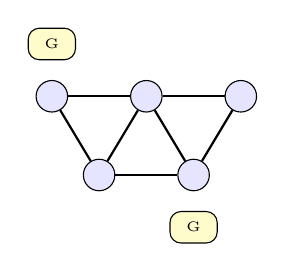
\begin{tikzpicture}[node distance=0.9cm and 0.9cm, every node/.style={font=\tiny}]
\tikzset{bus/.style={draw, circle, minimum size=0.4cm, fill=blue!10, inner sep=0pt}}
\tikzset{gen/.style={draw, rounded corners, fill=yellow!20, minimum width=0.6cm, minimum height=0.4cm, inner sep=1pt}}
\node[bus] (b1) {};  \node[gen, above=0.25cm of b1] {G};
\node[bus] (b2) at (1.2,0)  {};
\node[bus] (b3) at (0.6,-1) {};
\node[bus] (b4) at (1.8,-1) {}; \node[gen, below=0.25cm of b4] {G};
\node[bus] (b5) at (2.4,0)  {};
\draw[thick] (b1)--(b2); \draw[thick] (b1)--(b3);
\draw[thick] (b2)--(b3); \draw[thick] (b2)--(b4);
\draw[thick] (b3)--(b4); \draw[thick] (b2)--(b5);
\draw[thick] (b4)--(b5);
\end{tikzpicture}\\[0.3em]
\footnotesize Meshed. Multiple generators. 110--765 kV.
\column{0.5\textwidth}
\centering
\textbf{Distribution feeder}\\[0.4em]
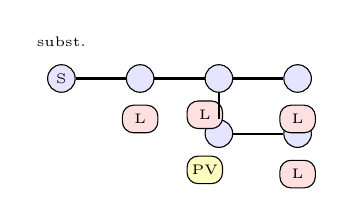
\begin{tikzpicture}[node distance=0.7cm and 0.7cm, every node/.style={font=\tiny}]
\tikzset{bus/.style={draw, circle, minimum size=0.35cm, fill=blue!10, inner sep=0pt}}
\tikzset{ld/.style={draw, rounded corners, fill=red!12, minimum width=0.45cm, minimum height=0.35cm, inner sep=1pt}}
\tikzset{pv/.style={draw, rounded corners, fill=yellow!25, minimum width=0.45cm, minimum height=0.35cm, inner sep=1pt}}
\node[bus] (s) {S}; \node[font=\tiny, above=0.1cm of s] {subst.};
\node[bus] (b1) at (1.0,0) {};
\node[bus] (b2) at (2.0,0) {};
\node[bus] (b3) at (3.0,0) {};
\node[bus] (b4) at (2.0,-0.7) {};
\node[bus] (b5) at (3.0,-0.7) {};
\node[ld, below=0.15cm of b1] {L};
\node[ld, below=0.15cm of b2.south west, xshift=-0.05cm] {L};
\node[ld, below=0.15cm of b3] {L};
\node[pv, below=0.15cm of b4.south west, xshift=-0.05cm] {PV};
\node[ld, below=0.15cm of b5] {L};
\draw[thick] (s)--(b1)--(b2)--(b3);
\draw[thick] (b2)--(b4)--(b5);
\end{tikzpicture}\\[0.3em]
\footnotesize Radial. One source. 0.4--35 kV. Many small loads + DER.
\end{columns}
\vspace{0.6em}
\begin{block}{Why we cannot just reuse L01 directly}
The math from L01 still applies in principle, but every \emph{practical} assumption (balanced phases, low R/X, mesh topology, stable convergence) is weaker or wrong on distribution feeders.
\end{block}
\end{frame}

% ============================================================
\begin{frame}{Side-by-side comparison}
\centering
\small
\begin{tabular}{lll}
\toprule
 & \textbf{Transmission} & \textbf{Distribution} \\
\midrule
Voltage level & 110 kV -- 765 kV & 0.4 kV -- 35 kV \\
Topology & Meshed (loops) & Radial (tree) \\
Line R/X ratio & 0.1 -- 0.3 & 1 -- 3 (sometimes higher) \\
Loads & Aggregated, balanced & Many small, often single-phase \\
Generators & Large central, three-phase & PV / BESS / EV, often single-phase \\
Phase symmetry & Usually fine & Rarely true \\
Direction of flow & One direction historically & Bi-directional with DER \\
Typical solver & Newton-Raphson (NR) & BFS, BFSW, sometimes NR \\
\bottomrule
\end{tabular}
\vspace{0.8em}
\begin{block}{Reading this table}
Every row is a reason this lecture exists. We will see each effect concretely on a small example before the lecture ends.
\end{block}
\end{frame}

% ============================================================
\begin{frame}{The R/X problem -- with numbers}
For a single radial line carrying load $P + jQ$ to the next bus, the voltage drop is approximately
\begin{equation*}
\Delta V = V_i - V_j \;\approx\; \frac{R \, P + X \, Q}{V} \quad (\text{small-angle, low-loss approximation})
\end{equation*}
\vspace{0.3em}
Take a load of $P = 1.0$ pu, $Q = 0.3$ pu at $V \approx 1$ pu:
\vspace{0.3em}
\centering
\small
\begin{tabular}{lccc}
\toprule
 & $R$ (pu) & $X$ (pu) & $\Delta V$ (pu) \\
\midrule
Transmission line & 0.01 & 0.10 & $0.01 + 0.03 = \textbf{0.04}$ \\
LV distribution feeder & 0.10 & 0.05 & $0.10 + 0.015 = \textbf{0.115}$ \\
\bottomrule
\end{tabular}
\vspace{0.6em}
\begin{alertblock}{The consequence}
On the LV feeder $\Delta V$ is \emph{three times larger} \emph{and} dominated by the active-power term. The classical ``$P$ moves $\theta$, $Q$ moves $|V|$'' decoupling from textbook transmission analysis no longer holds.
\end{alertblock}
\end{frame}

% ============================================================
\begin{frame}{Why this matters for solvers}
\begin{columns}[T]
\column{0.5\textwidth}
\textbf{Newton-Raphson assumes...}
\begin{itemize}
  \item Reasonable initial guess (flat start works)
  \item Well-conditioned Jacobian
  \item Modest voltage drops
  \item Mostly inductive lines (low R/X)
\end{itemize}
\vspace{0.4em}
On long, heavily-loaded LV feeders, the Jacobian can become ill-conditioned and NR may not converge from a flat start.
\column{0.5\textwidth}
\textbf{Specialized distribution methods exploit...}
\begin{itemize}
  \item Radial topology (a tree, not a graph)
  \item Single path from each bus to the source
  \item Easy KCL summation along that path
  \item No need to factor a large Jacobian
\end{itemize}
\vspace{0.4em}
\begin{block}{The most common is BFS}
Backward/Forward Sweep: walk the tree twice per iteration. Simple. Robust on long radial feeders.
\end{block}
\end{columns}
\end{frame}

% ============================================================
\section*{2. Radial topology and Backward/Forward Sweep}

\begin{frame}{What ``radial'' means}
\centering
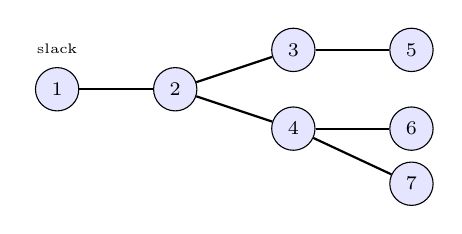
\begin{tikzpicture}[node distance=1.4cm and 1.4cm, every node/.style={font=\scriptsize}]
\tikzset{bus/.style={draw, circle, minimum size=0.55cm, fill=blue!10}}
\node[bus] (s) {1};
\node[font=\tiny, above=0.05cm of s] {slack};
\node[bus] (b2) at (1.5,0) {2};
\node[bus] (b3) at (3.0,0.5) {3};
\node[bus] (b4) at (3.0,-0.5) {4};
\node[bus] (b5) at (4.5,0.5) {5};
\node[bus] (b6) at (4.5,-0.5) {6};
\node[bus] (b7) at (4.5,-1.2) {7};
\draw[thick] (s)--(b2);
\draw[thick] (b2)--(b3);
\draw[thick] (b2)--(b4);
\draw[thick] (b3)--(b5);
\draw[thick] (b4)--(b6);
\draw[thick] (b4)--(b7);
\end{tikzpicture}
\vspace{0.8em}
\begin{columns}[T]
\column{0.5\textwidth}
\textbf{Properties of a radial network}
\begin{itemize}
  \item Exactly one path from any bus back to the slack
  \item No loops
  \item Each non-slack bus has exactly one ``parent''
  \item Looks like a tree rooted at the substation
\end{itemize}
\column{0.5\textwidth}
\textbf{Why this is exploitable}
\begin{itemize}
  \item Currents downstream of bus $k$ all flow through one branch
  \item KCL at each bus is a simple sum
  \item KVL along each branch is one equation
  \item No matrix inversion needed
\end{itemize}
\end{columns}
\end{frame}

% ============================================================
\begin{frame}{Backward/Forward Sweep: the intuition}
\centering
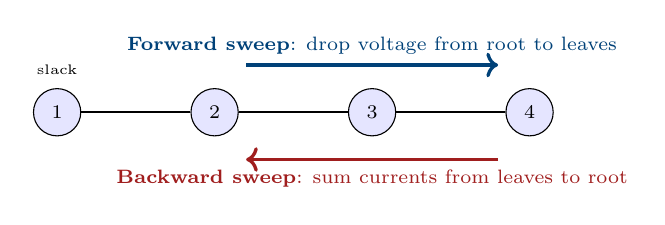
\begin{tikzpicture}[node distance=1.6cm and 1.6cm, every node/.style={font=\scriptsize}]
\tikzset{bus/.style={draw, circle, minimum size=0.6cm, fill=blue!10}}
\node[bus] (b1) {1};   \node[font=\tiny, above=0.05cm of b1] {slack};
\node[bus] (b2) at (2,0) {2};
\node[bus] (b3) at (4,0) {3};
\node[bus] (b4) at (6,0) {4};
\draw[thick] (b1)--(b2)--(b3)--(b4);
\draw[->, very thick, darkred] (5.6,-0.6) -- (2.4,-0.6) node[midway, below, font=\scriptsize]{\textbf{Backward sweep}: sum currents from leaves to root};
\draw[->, very thick, darkblue] (2.4,0.6) -- (5.6,0.6) node[midway, above, font=\scriptsize]{\textbf{Forward sweep}: drop voltage from root to leaves};
\end{tikzpicture}
\vspace{0.8em}
\begin{block}{Two-line summary}
\textbf{Backward:} given a voltage estimate, compute the load current at each bus and \emph{sum} currents flowing toward the substation.\\
\textbf{Forward:} given the branch currents, walk from the slack outward and \emph{subtract} the voltage drop on each branch.
\end{block}
\vspace{0.3em}
Repeat backward + forward until the voltage estimate stops changing.
\end{frame}

% ============================================================
\begin{frame}[fragile]{BFS algorithm in pseudocode}
\textbf{Inputs:} radial topology, line impedances $z_{ij}$, complex loads $S_i$, slack voltage $V_1$.\\
\textbf{Initialize:} $V_i \leftarrow V_1$ for all $i$ (flat start).
\vspace{0.4em}
\begin{lstlisting}[language=Python]
while not converged:
    # ---- Backward sweep ----
    # Walk from leaves to root, in reverse topological order
    for bus i in reverse_order:
        I_load_i = conj(S_i / V_i)
        I_branch[parent(i) -> i] = I_load_i + sum(I_branch[i -> child])

    # ---- Forward sweep ----
    # Walk from root outward, in topological order
    for bus j in forward_order (excluding slack):
        i = parent(j)
        V_j = V_i - z_ij * I_branch[i -> j]

    converged = max(|V_new - V_old|) < tol
\end{lstlisting}
\vspace{0.3em}
\begin{alertblock}{Why this works}
Radial structure guarantees \code{I\_branch[i $\rightarrow$ j]} is unique: only one path connects each bus to the slack.
\end{alertblock}
\end{frame}

% ============================================================
\section*{3. A worked BFS example}

\begin{frame}{4-bus radial feeder: setup}
\centering
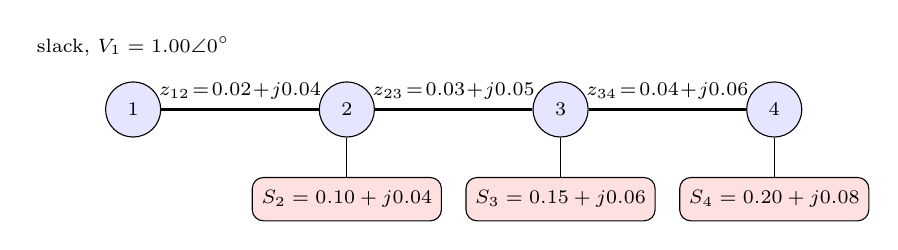
\begin{tikzpicture}[node distance=2.0cm and 2.0cm, every node/.style={font=\scriptsize}]
\tikzset{bus/.style={draw, circle, minimum size=0.7cm, fill=blue!10}}
\tikzset{ld/.style={draw, rounded corners, fill=red!12, minimum width=1.5cm, minimum height=0.55cm}}
\node[bus] (b1) {1};
\node[bus, right=of b1] (b2) {2};
\node[bus, right=of b2] (b3) {3};
\node[bus, right=of b3] (b4) {4};
\node[font=\scriptsize, above=0.2cm of b1] {slack, $V_1 = 1.00 \angle 0^\circ$};
\node[ld, below=0.5cm of b2] (l2) {$S_2 = 0.10 + j0.04$};
\node[ld, below=0.5cm of b3] (l3) {$S_3 = 0.15 + j0.06$};
\node[ld, below=0.5cm of b4] (l4) {$S_4 = 0.20 + j0.08$};
\draw[thick] (b1) -- node[above, font=\scriptsize]{$z_{12}\!=\!0.02\!+\!j0.04$} (b2);
\draw[thick] (b2) -- node[above, font=\scriptsize]{$z_{23}\!=\!0.03\!+\!j0.05$} (b3);
\draw[thick] (b3) -- node[above, font=\scriptsize]{$z_{34}\!=\!0.04\!+\!j0.06$} (b4);
\draw (b2)--(l2); \draw (b3)--(l3); \draw (b4)--(l4);
\end{tikzpicture}
\vspace{0.6em}
\begin{block}{All values are in per-unit on a common base}
Total load: $P = 0.45$ pu, $Q = 0.18$ pu. Lines are short and resistive (typical LV feeder). Flat start: $V_2 = V_3 = V_4 = 1.0$.
\end{block}
\end{frame}

% ============================================================
\begin{frame}{Iteration 1 -- Backward sweep}
With $V_i = 1.0$ everywhere, the load currents are $I^{\text{load}}_i = (S_i / V_i)^*$:
\vspace{0.3em}
\centering
\small
\begin{tabular}{lll}
\toprule
Bus & $S_i$ (pu) & $I^{\text{load}}_i$ (pu) \\
\midrule
2 & $0.10 + j0.04$ & $0.10 - j0.04$ \\
3 & $0.15 + j0.06$ & $0.15 - j0.06$ \\
4 & $0.20 + j0.08$ & $0.20 - j0.08$ \\
\bottomrule
\end{tabular}
\vspace{0.5em}
Branch currents accumulate from the leaf back to the slack:
\begin{align*}
I_{3\to 4} &= I^{\text{load}}_4 = 0.20 - j0.08 \\
I_{2\to 3} &= I^{\text{load}}_3 + I_{3\to 4} = 0.35 - j0.14 \\
I_{1\to 2} &= I^{\text{load}}_2 + I_{2\to 3} = 0.45 - j0.18
\end{align*}
\begin{block}{Sanity check}
$I_{1\to 2}$ matches total downstream load $0.45 - j0.18$. At flat start, branch currents are just summed load currents.
\end{block}
\end{frame}

% ============================================================
\begin{frame}{Iteration 1 -- Forward sweep}
Walk from the slack outward, dropping voltage by $z_{ij} \cdot I_{i \to j}$:
\vspace{0.3em}
\begin{align*}
V_2 &= V_1 - z_{12} \cdot I_{1\to 2}
     = 1.000 - (0.02 + j0.04)(0.45 - j0.18) \\
     &= 1.000 - (0.0162 + j0.0144) = 0.984 - j0.014 \\
V_3 &= V_2 - z_{23} \cdot I_{2\to 3}
     = 0.984 - j0.014 - (0.03 + j0.05)(0.35 - j0.14) \\
     &= 0.984 - j0.014 - (0.0175 + j0.0133) = 0.966 - j0.028 \\
V_4 &= V_3 - z_{34} \cdot I_{3\to 4}
     = 0.966 - j0.028 - (0.04 + j0.06)(0.20 - j0.08) \\
     &= 0.966 - j0.028 - (0.0128 + j0.0088) = 0.954 - j0.037
\end{align*}
\vspace{0.3em}
\centering
\small
\begin{tabular}{lcc}
\toprule
Bus & $V_i$ (complex pu) & $|V_i|$ (pu) \\
\midrule
2 & $0.984 - j0.014$ & 0.984 \\
3 & $0.966 - j0.028$ & 0.967 \\
4 & $0.954 - j0.037$ & 0.954 \\
\bottomrule
\end{tabular}
\end{frame}

% ============================================================
\begin{frame}{Convergence in a few sweeps}
\centering
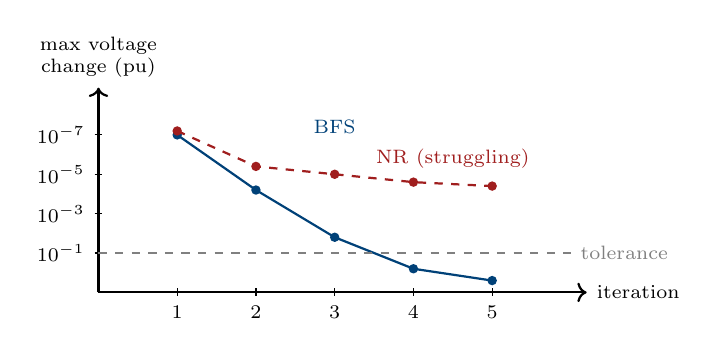
\begin{tikzpicture}[every node/.style={font=\scriptsize}]
\draw[->, thick] (0,0) -- (6.2,0) node[right]{iteration};
\draw[->, thick] (0,0) -- (0,2.6) node[above, align=center]{max voltage\\change (pu)};
% x-axis ticks
\draw (1,0.05)--(1,-0.05) node[below]{1};
\draw (2,0.05)--(2,-0.05) node[below]{2};
\draw (3,0.05)--(3,-0.05) node[below]{3};
\draw (4,0.05)--(4,-0.05) node[below]{4};
\draw (5,0.05)--(5,-0.05) node[below]{5};
% y-axis ticks
\draw (-0.05,0.5)--(0.05,0.5) node[left, xshift=-0.1cm]{$10^{-1}$};
\draw (-0.05,1.0)--(0.05,1.0) node[left, xshift=-0.1cm]{$10^{-3}$};
\draw (-0.05,1.5)--(0.05,1.5) node[left, xshift=-0.1cm]{$10^{-5}$};
\draw (-0.05,2.0)--(0.05,2.0) node[left, xshift=-0.1cm]{$10^{-7}$};
\draw[thick, darkblue] plot coordinates {(1,2.0) (2,1.3) (3,0.7) (4,0.3) (5,0.15)};
\foreach \p in {(1,2.0), (2,1.3), (3,0.7), (4,0.3), (5,0.15)} \fill[darkblue] \p circle (0.06);
\node[darkblue] at (3.0,2.1) {BFS};
\draw[thick, darkred, dashed] plot coordinates {(1,2.05) (2,1.6) (3,1.5) (4,1.4) (5,1.35)};
\foreach \p in {(1,2.05), (2,1.6), (3,1.5), (4,1.4), (5,1.35)} \fill[darkred] \p circle (0.06);
\node[darkred] at (4.5,1.7) {NR (struggling)};
\draw[dashed, gray] (0,0.5) -- (6.0,0.5) node[right, gray]{tolerance};
\end{tikzpicture}
\vspace{0.6em}
\begin{columns}[T]
\column{0.5\textwidth}
\textbf{BFS typically}
\begin{itemize}
  \item 3--6 iterations to $10^{-8}$
  \item Cheap per iteration (no Jacobian)
  \item Reliable on long radial feeders
\end{itemize}
\column{0.5\textwidth}
\textbf{NR on the same problem}
\begin{itemize}
  \item May not converge from flat start
  \item Each iteration more expensive
  \item Better on meshed transmission
\end{itemize}
\end{columns}
\vspace{0.2em}
\footnotesize\emph{Illustrative; exact convergence rate depends on R/X, loading, and topology.}
\end{frame}

% ============================================================
\begin{frame}[fragile]{When BFS beats NR (and when it does not)}
\centering
\small
\begin{tabular}{lcc}
\toprule
Scenario & BFS & NR \\
\midrule
Long radial LV feeder, heavy load & \checkitem & \warnitem \\
High R/X (e.g.\ 1--3) & \checkitem & \warnitem \\
Lightly-meshed distribution & \checkitem* & \checkitem \\
Heavily-meshed transmission & \warnitem & \checkitem \\
PV-rich feeder with reverse flow & \checkitem* & \checkitem \\
Need exact derivatives (sensitivity studies) & \warnitem & \checkitem \\
\bottomrule
\end{tabular}
\vspace{0.5em}
\footnotesize \checkitem*\ requires BFSW (Backward/Forward Sweep with Walks) or other generalizations.
\vspace{0.6em}
\begin{block}{In pandapower}
\begin{lstlisting}[language=Python, basicstyle=\ttfamily\scriptsize]
pp.runpp(net, algorithm="bfsw")   # backward/forward sweep with walks
pp.runpp(net, algorithm="nr")     # default Newton-Raphson
\end{lstlisting}
Try both on the same network. On a long LV feeder you will often see one converge while the other does not.
\end{block}
\end{frame}

% ============================================================
\section*{4. LinDistFlow: when a linear model is enough}

\begin{frame}{The exact branch equation}
For a radial branch from bus $i$ to bus $j$ carrying complex power $P_{ij} + jQ_{ij}$ at the sending end:
\begin{equation*}
|V_i|^2 - |V_j|^2 \;=\; 2\,(R_{ij}\,P_{ij} + X_{ij}\,Q_{ij}) \;-\; |Z_{ij}|^2 \cdot |I_{ij}|^2
\end{equation*}
Two terms:
\begin{itemize}
  \item $2(R P + X Q)$ -- the dominant ``voltage drop'' term, linear in $P, Q$.
  \item $|Z|^2 \cdot |I|^2$ -- the ``loss'' term, quadratic in current. Small when V is near 1 and losses are a few percent.
\end{itemize}
\vspace{0.5em}
\begin{block}{LinDistFlow (Baran \& Wu, 1989)}
Drop the loss term. Then linearize $|V_i|^2 - |V_j|^2 \approx 2(|V_i| - |V_j|)$ around $|V| \approx 1$:
\begin{equation*}
\boxed{\;|V_i| - |V_j| \;\approx\; R_{ij}\,P_{ij} + X_{ij}\,Q_{ij}\;}
\end{equation*}
A clean linear formula. Used everywhere in distribution planning and optimization.
\end{block}
\end{frame}

% ============================================================
\begin{frame}{LinDistFlow on the worked example}
Apply LinDistFlow to the same 4-bus feeder, using $P_{ij}, Q_{ij}$ = total downstream load on each branch:
\vspace{0.3em}
\centering
\small
\begin{tabular}{lcccc}
\toprule
Branch & $P_{ij}$ (pu) & $Q_{ij}$ (pu) & $\Delta V = RP + XQ$ & $|V_j|^{\text{LinDist}}$ \\
\midrule
$1 \to 2$ & 0.45 & 0.18 & $0.02(0.45)+0.04(0.18)\!=\!0.016$ & 0.984 \\
$2 \to 3$ & 0.35 & 0.14 & $0.03(0.35)+0.05(0.14)\!=\!0.017$ & 0.967 \\
$3 \to 4$ & 0.20 & 0.08 & $0.04(0.20)+0.06(0.08)\!=\!0.013$ & 0.954 \\
\bottomrule
\end{tabular}
\vspace{0.5em}
\centering
\small
\begin{tabular}{lcc}
\toprule
Bus & $|V|$ from BFS & $|V|$ from LinDistFlow \\
\midrule
2 & 0.984 & 0.984 \\
3 & 0.967 & 0.967 \\
4 & 0.954 & 0.954 \\
\bottomrule
\end{tabular}
\vspace{0.5em}
\begin{block}{Why they agree so well}
On this feeder, voltages are close to 1.0 pu and losses are a fraction of a percent. The neglected $|Z|^2|I|^2$ term is in the 4th decimal place.
\end{block}
\end{frame}

% ============================================================
\begin{frame}{When LinDistFlow is accurate, and when it lies}
\begin{columns}[T]
\column{0.5\textwidth}
\textbf{Accurate within $\sim 0.5\%$ when:}
\begin{itemize}
  \item All $|V_i| \in [0.95, 1.05]$
  \item Losses $<$ 2--3\% of total flow
  \item No large reverse flow
  \item No dominant $|I|^2$ heating
\end{itemize}
\column{0.5\textwidth}
\textbf{Becomes optimistic when:}
\begin{itemize}
  \item Heavy PV generation pushing voltages above 1.05
  \item Long feeder with $|V|$ near 0.92--0.93
  \item High line current $\rightarrow$ $|I|^2 R$ losses matter
  \item Capacitor banks switching $\rightarrow$ Q changes abruptly
\end{itemize}
\end{columns}
\vspace{0.5em}
\begin{block}{Where you will see it}
LinDistFlow underlies many distribution OPF formulations, DER siting/sizing problems, and Volt/VAR optimization. We will use BFS in this course because we want absolute voltage values, but the linear form is what makes large planning problems tractable.
\end{block}
\end{frame}

% ============================================================
\section*{5. DER on distribution feeders}

\begin{frame}{What DER changes}
\centering
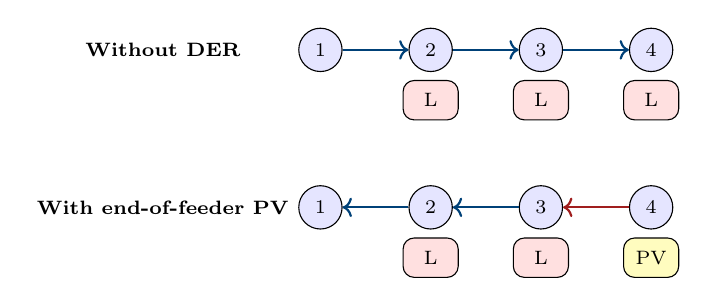
\begin{tikzpicture}[node distance=1.4cm and 1.4cm, every node/.style={font=\scriptsize}]
\tikzset{bus/.style={draw, circle, minimum size=0.55cm, fill=blue!10}}
\tikzset{src/.style={draw, rounded corners, fill=yellow!25, minimum width=0.7cm, minimum height=0.5cm}}
\tikzset{ld/.style={draw, rounded corners, fill=red!12, minimum width=0.7cm, minimum height=0.5cm}}

% Top: without PV
\node at (-2.0, 1.0) {\textbf{Without DER}};
\node[bus] (a1) at (0,1.0) {1};
\node[bus] (a2) at (1.4,1.0) {2};
\node[bus] (a3) at (2.8,1.0) {3};
\node[bus] (a4) at (4.2,1.0) {4};
\node[ld, below=0.1cm of a2] {L};
\node[ld, below=0.1cm of a3] {L};
\node[ld, below=0.1cm of a4] {L};
\draw[->, thick, darkblue] (a1)--(a2); \draw[->, thick, darkblue] (a2)--(a3); \draw[->, thick, darkblue] (a3)--(a4);

% Bottom: with PV
\node at (-2.0, -1.0) {\textbf{With end-of-feeder PV}};
\node[bus] (c1) at (0,-1.0) {1};
\node[bus] (c2) at (1.4,-1.0) {2};
\node[bus] (c3) at (2.8,-1.0) {3};
\node[bus] (c4) at (4.2,-1.0) {4};
\node[ld, below=0.1cm of c2] {L};
\node[ld, below=0.1cm of c3] {L};
\node[src, below=0.1cm of c4] {PV};
\draw[->, thick, darkblue] (c2)--(c1); \draw[->, thick, darkblue] (c3)--(c2);
\draw[->, thick, darkred] (c4)--(c3);
\end{tikzpicture}
\vspace{0.4em}
\begin{itemize}
  \item Without DER: power flows substation $\rightarrow$ loads. Voltage decreases away from substation.
  \item With heavy DER at the end of the feeder: power can flow \emph{toward} the substation. Voltage \emph{rises} near the DER.
\end{itemize}
\end{frame}

% ============================================================
\begin{frame}{Voltage rise -- a numerical example}
A 2-bus toy feeder, LV characteristics: $z = 0.05 + j0.05$ pu, $V_1 = 1.00$.
\vspace{0.3em}
\centering
\small
\begin{tabular}{lccc}
\toprule
Case & Net injection at bus 2 & $\Delta V = (RP + XQ)/V$ & $|V_2|$ \\
\midrule
(a) 0.5 pu load only & $-0.50$ pu & $+0.025$ & \textbf{0.975} pu \\
(b) 0.5 pu PV, 0.5 pu load (offset) & $\phantom{-}0.00$ pu & $\phantom{+}0.000$ & \textbf{1.000} pu \\
(c) 1.5 pu PV, 0.5 pu load (export 1.0) & $+1.00$ pu & $-0.050$ & \textbf{1.050} pu \\
(d) 2.0 pu PV, 0.5 pu load (export 1.5) & $+1.50$ pu & $-0.075$ & \textbf{1.075} pu \\
\bottomrule
\end{tabular}
\vspace{0.6em}
\begin{alertblock}{The pattern}
Case (a) is the classical low-voltage problem: load $\rightarrow$ voltage drops.\\
Case (d) is the modern high-voltage problem: PV $\rightarrow$ voltage rises past 1.05 pu.\\
\textbf{Same feeder, opposite violations.} A simple ``low-voltage check'' is no longer enough.
\end{alertblock}
\end{frame}

% ============================================================
\begin{frame}{Reverse power flow and what it breaks}
\begin{columns}[T]
\column{0.55\textwidth}
\textbf{When DER injection at a bus exceeds local load,} net power flows \emph{toward} the substation. Several consequences:
\begin{itemize}
  \item Voltage rises along the upstream path.
  \item Some protection relays assume one-directional flow.
  \item Transformer tap controllers may move the wrong way.
  \item Loss calculations need to be reconsidered.
\end{itemize}
\column{0.42\textwidth}
\begin{block}{Magnitude in practice}
At 30--50\% PV penetration on a typical LV feeder, the substation can already see negative net flow at midday on clear weekends.
\end{block}
\begin{alertblock}{Connection to this course}
Reverse flow + voltage rise = a violation mode the N-1 screening model must learn. Week 4 of the project labels both kinds.
\end{alertblock}
\end{columns}
\end{frame}

% ============================================================
\begin{frame}{Hosting capacity in one slide}
\textbf{Question:} how much DER can be added to a feeder before \emph{any} voltage or thermal limit is violated?
\vspace{0.4em}
\centering
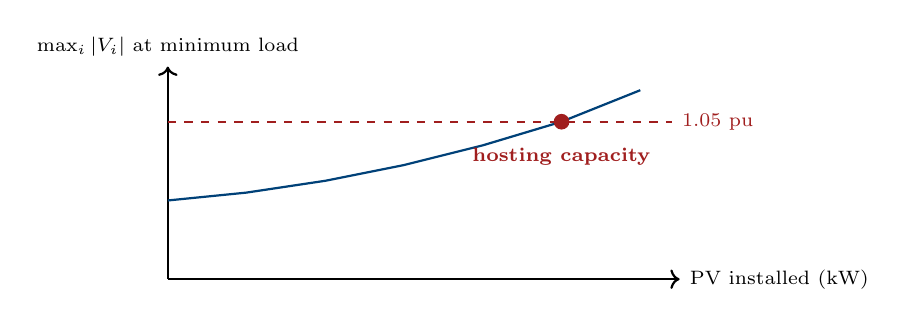
\begin{tikzpicture}[every node/.style={font=\scriptsize}]
\draw[->, thick] (0,0)--(6.5,0) node[right]{PV installed (kW)};
\draw[->, thick] (0,0)--(0,2.7) node[above]{$\max_i |V_i|$ at minimum load};
\draw[dashed, darkred, thick] (0,2.0)--(6.4,2.0) node[right, darkred]{1.05 pu};
\draw[thick, darkblue] plot coordinates {(0,1.0) (1,1.10) (2,1.25) (3,1.45) (4,1.7) (5,2.0) (6,2.4)};
\node[circle, fill=darkred, inner sep=2pt] (hc) at (5,2.0) {};
\node[darkred, below=0.1cm of hc] {\textbf{hosting capacity}};
\end{tikzpicture}
\vspace{0.5em}
\begin{block}{Definitions}
\begin{itemize}
  \item \textbf{Hosting capacity} = the PV size at which the first constraint becomes binding under the worst-case operating condition (typically: maximum PV, minimum load).
  \item It is determined by either voltage rise or thermal overload, whichever comes first.
  \item Computing it requires the same N-1-style PF scans we will use in Weeks 3--4 of the project.
\end{itemize}
\end{block}
\end{frame}

% ============================================================
\section*{6. Microgrids and the bridge to L04}

\begin{frame}{Microgrid = distribution + control boundary}
\centering
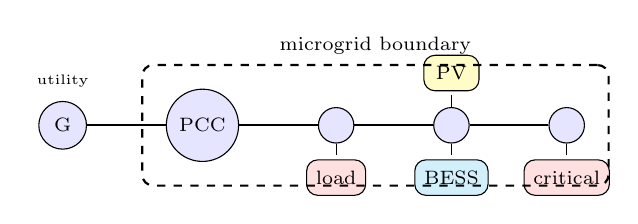
\begin{tikzpicture}[node distance=1.0cm and 1.0cm, every node/.style={font=\scriptsize}]
\tikzset{bus/.style={draw, circle, minimum size=0.45cm, fill=blue!10}}
\tikzset{src/.style={draw, rounded corners, fill=yellow!22, minimum width=0.7cm, minimum height=0.45cm}}
\tikzset{ld/.style={draw, rounded corners, fill=red!12, minimum width=0.7cm, minimum height=0.45cm}}
\tikzset{bess/.style={draw, rounded corners, fill=cyan!18, minimum width=0.7cm, minimum height=0.45cm}}
\node[bus] (grid) {G};
\node[font=\tiny, above=0.05cm of grid] {utility};
\node[bus, right=of grid] (pcc) {PCC};
\node[bus, right=of pcc] (b1) {};
\node[bus, right=of b1] (b2) {};
\node[bus, right=of b2] (b3) {};
\node[src, above=0.2cm of b2] {PV};
\node[bess, below=0.2cm of b2] {BESS};
\node[ld, below=0.2cm of b1] {load};
\node[ld, below=0.2cm of b3] {critical};
\draw[thick] (grid)--(pcc)--(b1)--(b2)--(b3);
\draw (b2.north)--++(0,0.15);
\draw (b2.south)--++(0,-0.15);
\draw (b1.south)--++(0,-0.15);
\draw (b3.south)--++(0,-0.15);
\node[draw, dashed, thick, rounded corners, fit=(pcc)(b1)(b2)(b3), inner sep=0.3cm, label=above:{microgrid boundary}] {};
\end{tikzpicture}
\vspace{0.6em}
\begin{block}{What ``microgrid'' adds on top of a distribution feeder}
\begin{itemize}
  \item Defined electrical boundary at the Point of Common Coupling (PCC).
  \item Internal generation that can support load when the utility is disconnected.
  \item Supervisory control (energy management system).
  \item Often: critical loads with higher reliability requirements.
\end{itemize}
\end{block}
\end{frame}

% ============================================================
\begin{frame}{Why distribution is rarely truly balanced}
\centering
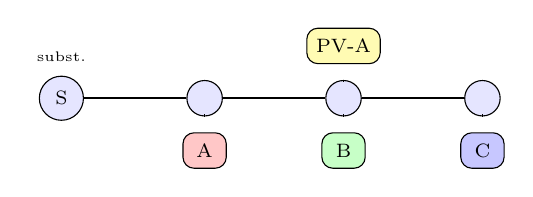
\begin{tikzpicture}[node distance=1.1cm and 1.3cm, every node/.style={font=\scriptsize}]
\tikzset{bus/.style={draw, circle, minimum size=0.45cm, fill=blue!10}}
\tikzset{ph/.style={draw, rounded corners, minimum width=0.55cm, minimum height=0.45cm}}
\node[bus] (s) {S}; \node[font=\tiny, above=0.05cm of s] {subst.};
\node[bus, right=of s] (b1) {};
\node[bus, right=of b1] (b2) {};
\node[bus, right=of b2] (b3) {};
\node[ph, fill=red!22, below=0.2cm of b1] {A};
\node[ph, fill=green!22, below=0.2cm of b2] {B};
\node[ph, fill=blue!22, below=0.2cm of b3] {C};
\node[ph, fill=yellow!30, above=0.2cm of b2] {PV-A};
\draw[thick] (s)--(b1)--(b2)--(b3);
\draw (b1)--++(0,-0.2);
\draw (b2)--++(0,-0.2);
\draw (b3)--++(0,-0.2);
\draw (b2)--++(0,0.2);
\end{tikzpicture}
\vspace{0.4em}
\textbf{Sources of phase asymmetry on LV / microgrid feeders:}
\begin{itemize}
  \item Single-phase loads (most residential consumers connect to one phase only).
  \item Single-phase rooftop PV (the inverter is connected to the homeowner's phase).
  \item Single-phase EV chargers, water heaters, ovens.
  \item Untransposed lines -- transposition is rarely worth the cost at LV.
  \item Asymmetric three-phase loads (one phase under heavy use, others idle).
\end{itemize}
\vspace{0.4em}
\begin{alertblock}{Implication}
Phase A could drop to 0.92 pu while phase B sits at 1.01 pu and phase C at 1.03 pu. \emph{Average} voltage looks fine. Balanced power flow happily reports ``no violation''. Phase A is in violation.
\end{alertblock}
\end{frame}

% ============================================================
\begin{frame}{Teaser of L04}
\begin{columns}[T]
\column{0.55\textwidth}
\textbf{What L04 will add to today's machinery:}
\begin{itemize}
  \item Symmetrical components: positive, negative, zero.
  \item Sequence-domain formulation of the PF.
  \item Voltage Unbalance Factor (VUF).
  \item \code{pandapower.runpp\_3ph} as the practical solver.
  \item Five violation types (incl.\ VUF).
\end{itemize}
\column{0.42\textwidth}
\begin{block}{What stays from L02}
\begin{itemize}
  \item Radial topology still simplifies things.
  \item BFS generalizes to three-phase.
  \item Voltage rise behavior still applies per-phase.
  \item Hosting capacity becomes per-phase.
\end{itemize}
\end{block}
\end{columns}
\vspace{0.5em}
\begin{block}{Bridge}
L02 said: ``transmission tools do not transfer to distribution.'' L04 will say: ``single-phase distribution tools do not transfer to phase-aware distribution.'' Same kind of failure of an unstated assumption.
\end{block}
\end{frame}

% ============================================================
\section*{7. Homework and recap}

\begin{frame}{Homework}
\begin{block}{Required}
\begin{enumerate}
  \item Reproduce the 4-bus radial example in pandapower. Use \code{pp.create\_line\_from\_parameters} with $R, X$ consistent with the per-unit values in the slides.
  \item Run both \code{pp.runpp(net, algorithm="bfsw")} and \code{pp.runpp(net, algorithm="nr")}. Confirm \code{net.converged} for both and verify $|V_i|$ matches the worked example to 3 decimal places.
  \item Multiply all line impedances by 5. Re-run. Which bus moves the most? Why?
  \item Replace the load at bus 4 with a 1.0 pu PV \code{sgen}. Find the smallest PV injection that pushes $|V_4|$ above 1.05.
\end{enumerate}
\end{block}
\begin{block}{Optional}
\begin{enumerate}
  \item Implement BFS yourself in $\sim$30 lines of \code{numpy} and compare to pandapower's \code{bfsw}.
  \item Plot the voltage profile $|V_i|$ vs bus index for load levels 0\%, 50\%, 100\%, 150\% of the slide values.
  \item Find the hosting capacity (max PV at bus 4 before any violation) under the worst-case minimum load.
\end{enumerate}
\end{block}
\end{frame}

% ============================================================
\begin{frame}{Exit checklist}
\begin{enumerate}
  \item \checkitem I can explain in one sentence why transmission solvers struggle on distribution feeders.
  \item \checkitem I can sketch the side-by-side topology of a transmission vs distribution network.
  \item \checkitem I can write the simplified voltage drop $\Delta V = (RP + XQ)/V$ and explain when it lies.
  \item \checkitem I can describe one backward sweep and one forward sweep in BFS on a small radial feeder.
  \item \checkitem I can choose between \code{algorithm="nr"} and \code{algorithm="bfsw"} for a given network.
  \item \checkitem I can describe how end-of-feeder PV causes voltage rise.
  \item \checkitem I can define hosting capacity in two sentences.
  \item \checkitem I know exactly which assumption from L02 will break in L04 (single-phase equivalent).
\end{enumerate}
\end{frame}

% ============================================================
\begin{frame}{References}
\footnotesize
\begin{itemize}
  \item \textbf{Kersting,} \emph{Distribution System Modeling and Analysis} (4th ed., 2017). The canonical distribution PF textbook.
  \item \textbf{Baran \& Wu, 1989.} \emph{Optimal Capacitor Placement on Radial Distribution Systems}, IEEE TPD. The DistFlow / LinDistFlow paper.
  \item \textbf{Cespedes, 1990.} \emph{New Method for the Analysis of Distribution Networks}, IEEE TPD. Classical BFS reference.
  \item \textbf{Shirmohammadi et al., 1988.} \emph{A Compensation-Based Power Flow Method for Weakly Meshed Distribution Networks}, IEEE TPS.
  \item \textbf{Bollen \& Hassan,} \emph{Integration of Distributed Generation in the Power System} (Wiley, 2011). Voltage rise, hosting capacity.
  \item \textbf{IEEE Std 1547-2018}, \emph{Standard for Interconnection of DER}. Voltage and frequency ride-through requirements.
  \item \textbf{pandapower docs:} \url{https://pandapower.readthedocs.io} -- look for ``BFSW'' under power-flow algorithms.
\end{itemize}
\end{frame}

\end{document}
